\documentclass{beamer}
\usetheme{Warsaw}

\usepackage{amsmath}
\usepackage{amsfonts}
\usepackage{amssymb}
\usepackage{color}
\usepackage{cancel}

\newcommand{\bi}{\begin{itemize}}
\newcommand{\ei}{\end{itemize}}

\newcommand{\Ex}{\mathbb{E}}
\newcommand{\PDies}{\mathsf{D}}
\newcommand{\PLives}{\cancel{\PDies}}



\title{HARK: Open Source Tools for\\ Heterogeneous Agents Modeling}

\author{Matthew N. White}

\institute{University of Delaware}

\begin{document}

\begin{frame}
\maketitle
\end{frame}


\begin{frame}
\frametitle{Introduction to Dynamic Economic Models}

\begin{block}{Elements of a dynamic economic model:}
\bi
\item Situations agent(s) can be in: the \textbf{state space}

\item Choices agent(s) can make: the \textbf{control space}

\item Constraints agent(s) face when making choice

\item The nature of risks agent(s) face: the \textbf{shock distribution}

\item How those combine to yield tomorrow's state: \textbf{dynamics}

\item How agents feel about sequences of those: \textbf{preferences}

\item How agents \textbf{process information} and/or \textbf{make choice}

\ei
\end{block}

\end{frame}


\begin{frame}
\frametitle{Classification of Dynamic Economic Models}

\begin{block}{The nature of time:}
\bi
\item \textbf{Discrete} vs \textbf{continuous} time

\item \textbf{Finite} vs \textbf{infinite} horizon
\ei
\end{block}


\begin{block}{Representative vs Heterogeneous Agents}
\bi
\item In some models, one agent can stand in for many-- the \textbf{representative consumer} or \textbf{representative firm}

\item In others, shocks introduce \textit{ex post} heterogeneity
\ei
\end{block}

\end{frame}


\begin{frame}
\frametitle{Classification of Dynamic Economic Models}


\begin{block}{Equilibrium conditions:}
\bi
\item Agents solve their problem taking dynamics as \textbf{exogenous}

\item But some aspects of dynamics are \textbf{endogenous} to controls and states of agents collectively

\item \textbf{Information processing} includes \textbf{beliefs} about dynamics

\item \textbf{Equilibrium:} beliefs ``consistent'' with actual dynamics

\ei
\end{block}

\end{frame}



\begin{frame}
\frametitle{Getting Started in HA Macro in Ten Easy Years}

\begin{block}{Required knowledge to enter heterogeneous agents macro:}
\bi
\item Economic modeling (and history thereof)

\item Programming / software development

\item Numeric methods: optimization, rootfinding, interpolation...

\item Dynamic solution methodology

\item ``Trade secrets'' or ``occult knowledge''
\ei
\end{block}

\end{frame}


\begin{frame}
\frametitle{Getting Started in HA Macro in Ten Easy Years}

\begin{block}{Actually taught in economics PhD programs:}
\bi
\item \textcolor{red}{Economic modeling (and history thereof)}

\item \textcolor{gray}{Programming / software development}

\item Numeric methods: optimization, rootfinding, interpolation...

\item Dynamic solution methodology

\item \textcolor{gray}{``Trade secrets'' or ``occult knowledge''}
\ei
\end{block}

\end{frame}



\begin{frame}
\frametitle{Current State of HA Macro Modeling}

\begin{block}{How programming HA models is done today:}
\bi
\item Written for today, for one particular purpose

\item Everything is bespoke and handcrafted

\item Documentation is missing or apocryphal

\item Like econometrics circa 1970

\ei
\end{block}



\begin{block}{Strategies for HA model programming:}
\begin{enumerate}
\item Inherit codebase from your adviser('s adviser), repurpose

\item Re-reinvent the wheel / divine the secrets

\item Engage in ``duct tape coding''
\end{enumerate}
\end{block}


\end{frame}



\begin{frame}
\frametitle{Current State of HA Macro Modeling}

\begin{block}{Why are things done this way?}
\bi
\item PhD program inertia / limited bandwidth

\item Keep safe the secret of the secret sauce

\item Hide the rat droppings

\item Don't want to know how sausage is made
\ei

\end{block}
\end{frame}


\begin{frame}
\frametitle{Solution: HARK}

\begin{block}{Heterogeneous Agents Resources \& toolKit:}
\bi
\item Modular, extensible, interoperable, open source toolkit for solving discrete time heterogeneous agents models

\item For ``HA macro'' and ``structural micro'' models

\item Common framework for representing agents, environments, etc 

\item Dynamics, behavior, aggregation, and beliefs are modular

\item ``Model tree'' based on class inheritance
\ei
\end{block}

\end{frame}


\begin{frame}
\frametitle{Goals of HARK}

\begin{block}{HARK intended to make it \textbf{much} easier to...}
  \bi
\item Enter the world of HA modeling: reduce barriers

\item Teach HA methods and techniques (with hands-on exercises)

\item Compare models to each other: interoperability

\item Add new models and features: extensibility

\item Mix-and-match components: modularity
  \ei
\end{block}

\end{frame}



\begin{frame}{Goals of HARK}

\begin{block}{Ultimate goals of HARK:}
\bi
\item Accelerate development of models for research and policymaking

\item Bridge gaps among rational expectations, behavioral, ``agent-based'' modeling worlds

\item And between ``HA macro'' and ``structural micro''

\item Make code audits feasible/expected in refereeing

\ei
\end{block}
\end{frame}


\begin{frame}
\frametitle{Contents of HARK}

\begin{block}{Stuff in HARK, generally:}
\bi
\item Broadly useful numeric tools

\item Superclass for representing agents: \texttt{AgentType}

\item ...and environments they interact in: \texttt{Market}

\item Ever-expanding ``model tree'' as subclasses

\item In dev: documentation and tutorial notebooks
\ei

\end{block}
\end{frame}



\begin{frame}

\begin{center}
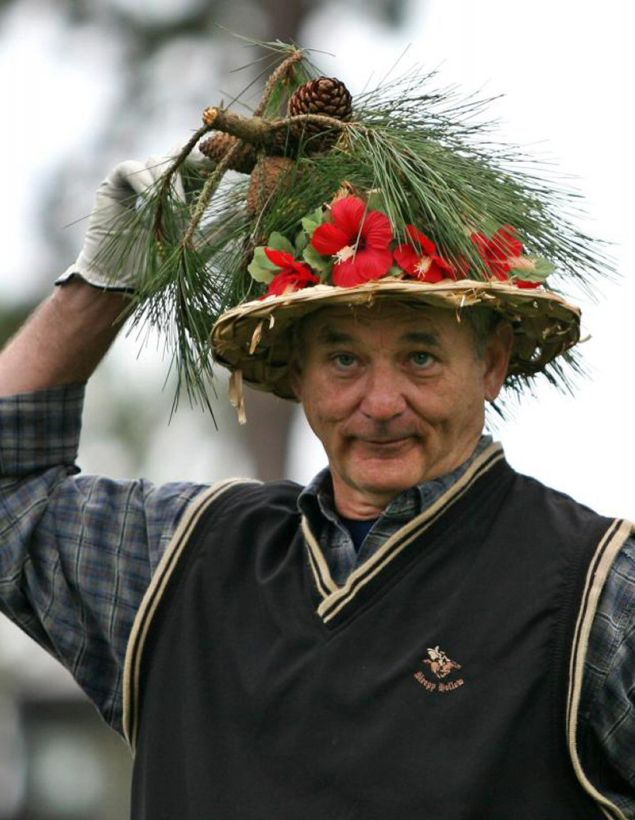
\includegraphics[scale=0.3]{BillMurray.jpg}
\end{center}

\end{frame}



\begin{frame}
\frametitle{HARK's Superclass for Agents: \texttt{AgentType}}

\begin{block}{The \texttt{AgentType} class:}
\bi
\item General purpose class for representing economic agents

\item Each model creates a subclass of \texttt{AgentType}
  \bi
  \item e.g. \texttt{PerfForesightConsumerType}
  \ei
\item Key method: \texttt{solve()}
    
\item Just a universal backward induction loop...

\item ...that lets different models ``play nicely'' together

\item Complex models extend basic ones through class inheritance
\ei

\end{block}
\end{frame}



\begin{frame}
\frametitle{Specifying a ``Microeconomic'' Model in HARK}

\begin{block}{Elements to specify a subclass of \texttt{AgentType}:}
\bi
\item What variables/objects agent needs to solve \textit{one period} of his problem, and whether those things vary over time: \texttt{time\_inv} and \texttt{time\_vary}

\item How to solve the one period problem, given current variables objects and solution to next period's problem: \texttt{solveOnePeriod}

\item How to behave at the end of time, or as an initial solution guess: \texttt{solveTerminal}
\ei
\end{block}
\end{frame}


\begin{frame}
\frametitle{Specifying a ``Microeconomic'' Model in HARK}

\begin{block}{Elements to specify an instance of an \texttt{AgentType} subclass:}
\bi
\item What is the nature of time? Lifecycle? Infinite horizon? Finitely repeated loop? \texttt{cycles} and \texttt{T\_cycle}

\item What values do variables named in \texttt{time\_vary} take on in each period of the ``cycle''?

\item What values do variables named in \texttt{time\_inv} take on?

\item How many agents of this ``type''? \texttt{AgentCount}

\ei

\end{block}
\end{frame}


\begin{frame}
  \frametitle{Example Model: Basic Consumption-Saving}

  Consumption-saving model with idiosyncratic permanent and transitory shocks to income (normalized format):

  \begin{equation*}
    u(c) = c^{1-\rho}/(1-\rho).
  \end{equation*}
  \begin{equation*}
    v_t(m_t) = \max_{c_t} u(c_t) + \beta \PLives_t \Ex_t \left[(\psi_{t+1} \Gamma_{t+1})^{1-\rho} v_{t+1}(m_{t+1}) \right] \text{ s.t. }
  \end{equation*}
  \begin{equation*}
    a_t = m_t - c_t, \hspace{0.5cm} a_t \geq \underline{a},
  \end{equation*}
  \begin{equation*}
    m_{t+1} = R/(\Gamma_{t+1} \psi_{t+1}) a_t + \theta_{t+1}, 
  \end{equation*}
  \begin{equation*}
    \psi_{t+1},\theta_{t+1} \sim F_{t+1}, \hspace{0.25cm} \Ex[\psi_{t+1}] = 1.
  \end{equation*}

\end{frame}



\begin{frame}
\frametitle{Example \texttt{AgentType} Subclass: \texttt{IndShockConsumerType}}

\begin{block}{Mapping from model to attributes named in \texttt{time\_inv}:}
\bi
\item Discount factor $\beta \longrightarrow$ \texttt{DiscFac}

\item Relative risk aversion $\rho \longrightarrow$ \texttt{CRRA}

\item Risk-free interest rate $R \longrightarrow$ \texttt{Rfree}

\item Artificial borrowing constraint $\underline{a} \longrightarrow$ \texttt{BoroCnstArt}
\ei
\end{block}


\begin{block}{Mapping from model to attributes named in \texttt{time\_vary}:}
\bi
\item Survival probability $\PLives_{t+1} \longrightarrow$ \texttt{LivPrb} 

\item Permanent income growth factor $\Gamma_{t+1} \longrightarrow$ \texttt{PermGroFac}

\item Distribution of perm and trans income shocks $F_{t+1} \longrightarrow$ \texttt{IncomeDstn}
\ei

\end{block}
\end{frame}


\begin{frame}
  \frametitle{\texttt{IndShockConsumerType} Consumption Function}
  \begin{center}
    \includegraphics[scale=0.65]{IndShockcFunc.pdf}
  \end{center}
\end{frame}


\begin{frame}
  \frametitle{Object-Oriented Solution Methods}
  \begin{itemize}
  \item ``Parent'' models in HARK are special cases of ``child'' models

  \item Solvers in HARK are object classes that act (a lot) like functions

  \item Child models inherit solver class from parent...
    
  \item ...and then add or change its methods as needed
  \end{itemize}
\end{frame}


\begin{frame}\
  \frametitle{Consumption-Saving Model Tree}
  \begin{center}
    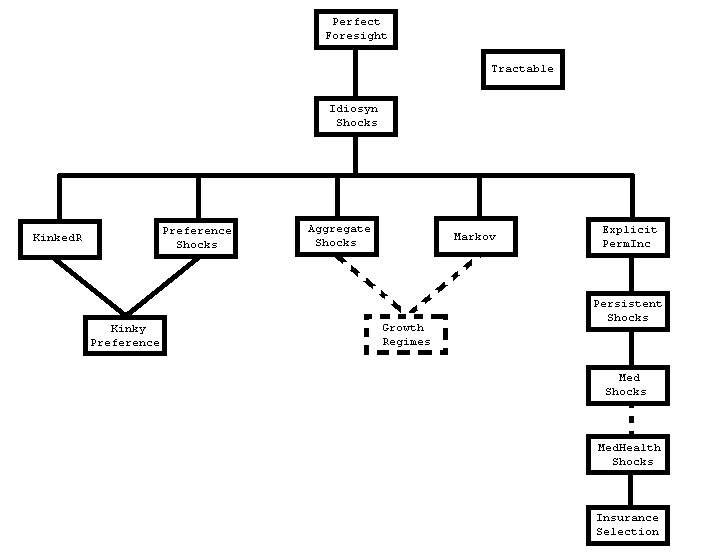
\includegraphics[scale=0.5]{NamesModelTree.png}
  \end{center}
\end{frame}


\begin{frame}
  \frametitle{Consumption-Saving Model Tree}
  \begin{center}
    \includegraphics[scale=0.5]{TreeHighlight2.png}
  \end{center}
\end{frame}

\begin{frame}
  \frametitle{Consumption-Saving Model Tree}
  \begin{center}
    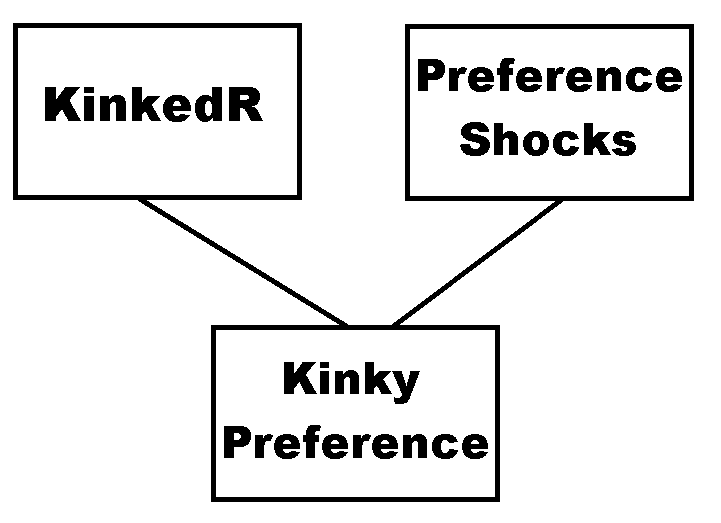
\includegraphics[scale=0.5]{TreeZoom2.png}
  \end{center}
\end{frame}


\begin{frame}
  \frametitle{Kinked R: Costly Borrowing (1/3)}
  Make one small adjustment to idiosyncratic income shocks model: interest rate on borrowing is higher than rate on saving.

  \begin{eqnarray*}
    u(c) &=& \frac{c^{1-\rho}}{1-\rho}, \\
    v(m_t) &=& \max_{c_t} u(c_t) + \beta \PLives_{t+1} \Ex [v_{t+1}(m_{t+1}) ], \\
    a_t &=& m_t - c_t, \qquad a_t \geq \underline{a}, \\
    m_{t+1} &=& R/(\Gamma_{t+1} \psi_{t+1}) a_t + \theta_{t+1}, \\
   \psi_{t+1},\theta_{t+1} \sim F_{t+1}, & & \Ex[\psi_{t+1}] = 1, \\
    R &=& \begin{cases}
      R_{boro} & \text{if  } a_t < 0 \\
      R_{save} & \text{if  } a_t > 0
    \end{cases}, \qquad R_{boro} \geq R_{save}.
  \end{eqnarray*}
\end{frame}


\begin{frame}
  \frametitle{Kinked R: Costly Borrowing (2/3)}
  \texttt{ConsKinkedRsolver} inherits from \texttt{ConsIndShockSolver}

  \begin{block}{Additions to \texttt{\_\_init\_\_} method:}
    \begin{itemize}
    \item Store new attributes \texttt{Rboro} and \texttt{Rsave}
    \end{itemize}
  \end{block}
  \begin{block}{Additions to \texttt{prepareToCalcEndOfPrdvP}:}
    \begin{itemize}
    \item Four lines to use correct value of $R$ for each value of $a_t$

    \item One line to apply that change to calculation of $m_{t+1}$

    \item Three lines to recalculate minimum MPC and human wealth
    \end{itemize}
  \end{block}
\end{frame}


\begin{frame}
  \frametitle{Kinked R: Costly Borrowing (3/3)}
  \begin{center}
    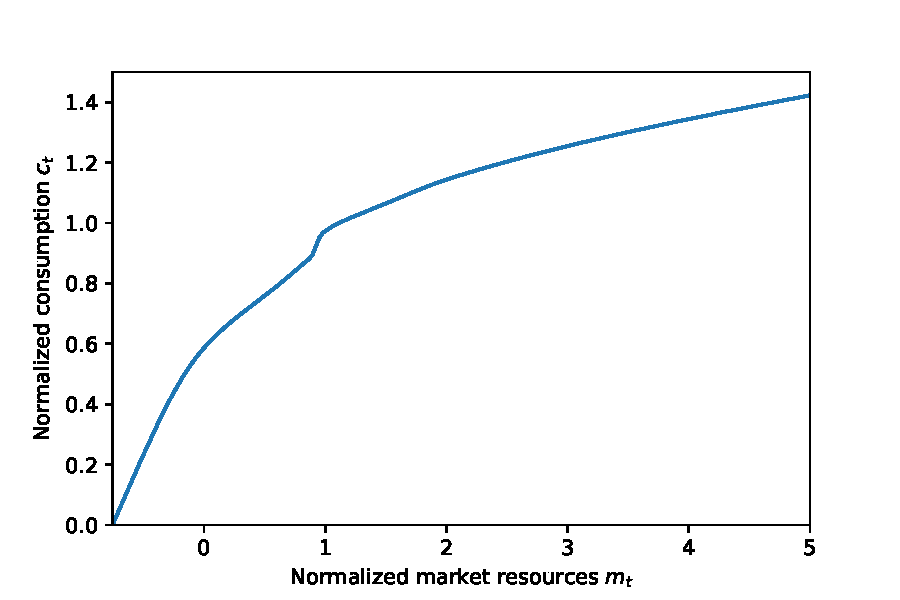
\includegraphics[scale=0.75]{KinkedRcFunc.pdf}
  \end{center}
\end{frame}



\begin{frame}
  \frametitle{Marginal Utility Shocks (1/3)}
  Consider another small modification to \texttt{IndShockModel}:
  \bi
\item Multiplicative (idiosyncratic) shocks to utility each period.

\item Consumption ``more valuable'' in some periods than others.
  \ei
  \begin{eqnarray*}
    u(c;\eta) &=& \eta \frac{c^{1-\rho}}{1-\rho}, \qquad \eta_t \sim F_{\eta}, \\
    v(m_t,\eta_t) &=& \max_{c_t} u(c_t;\eta_t) + \beta \PLives_{t+1} \Ex [v_{t+1}(m_{t+1}) ], \\
    a_t &=& m_t - c_t, \qquad a_t \geq \underline{a}, \\
    m_{t+1} &=& R/(\Gamma_{t+1} \psi_{t+1}) a_t + \theta_{t+1}, \\
    \psi_{t+1},\theta_{t+1} \sim F_{t+1}, & & \Ex[\psi_{t+1}] = 1. \\
  \end{eqnarray*}
\end{frame}


\begin{frame}
  \frametitle{Marginal Utility Shocks (2/3)}
  \texttt{ConsPrefShockSolver} inherits from \texttt{ConsIndShockSolver}

  \begin{block}{Additions to \texttt{\_\_init\_\_} method:}
    \begin{itemize}
    \item 2 lines: Store preference shock distribution \texttt{PrefShkDstn}
    \end{itemize}
  \end{block}

  \begin{block}{Replace \texttt{getPointsForInterpolation}}
    \begin{itemize}
    \item 8 lines: Values of $c_t$ and $m_t$ for each $\eta_t$ in \texttt{PrefShkDstn}
    \end{itemize}
  \end{block}

  \begin{block}{Replace \texttt{usePointsForInterpolation}}
    \begin{itemize}
    \item 6 lines: Construct \texttt{cFunc} as a \texttt{LinearInterpOnInterp1D}

    \item 6 lines: Make \texttt{vPfunc} by integrating marginal utility across $\eta_t$
    \end{itemize}
  \end{block}
\end{frame}

\begin{frame}
  \frametitle{Marginal Utility Shocks (2/3)}
  \begin{center}
    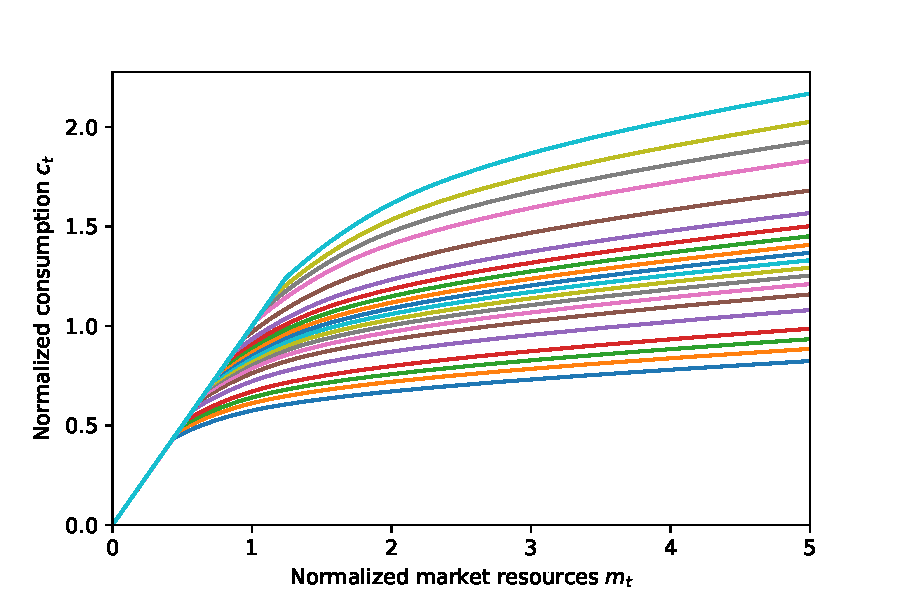
\includegraphics[scale=0.75]{PrefShockcFunc.pdf}
  \end{center}
\end{frame}


\begin{frame}
  \frametitle{Combination Inheritance: ``Kinky Preferences'' (1/4)}
  Combine those two extensions to \texttt{IndShockModel}:
  \begin{itemize}
  \item Borrowing has higher interest rate than saving...

  \item ...and there are shocks to marginal utility

  \item HARK makes this pretty easy
  \end{itemize}
\end{frame}


\begin{frame}
  \frametitle{Combination Inheritance: ``Kinky Preferences'' (2/4)}
  \begin{eqnarray*}
    u(c,\eta) &=& \eta \frac{c^{1-\rho}}{1-\rho}, \qquad \eta_t \sim F_{\eta},\\
    v(m_t,\eta_t) &=& \max_{c_t} u(c_t) + \beta \PLives_{t+1} \Ex [v_{t+1}(m_{t+1}) ], \\
    a_t &=& m_t - c_t, \qquad a_t \geq \underline{a}, \\
    m_{t+1} &=& R/(\Gamma_{t+1} \psi_{t+1}) a_t + \theta_{t+1}, \\
    \psi_{t+1},\theta_{t+1} \sim F_{t+1}, & & \Ex[\psi_{t+1}] = 1, \\
    R &=& \begin{cases}
      R_{boro} & \text{if  } a_t < 0 \\
      R_{save} & \text{if  } a_t > 0
    \end{cases}, \qquad R_{boro} \geq R_{save}.
  \end{eqnarray*}
\end{frame}



\begin{frame}
  \frametitle{Combination Inheritance: ``Kinky Preferences'' (3/4)}
   
Entirety of the code for the \texttt{ConsKinkyPrefSolver}:

\vspace{1cm}

  \scriptsize{
    \texttt{
      class ConsKinkyPrefSolver(ConsPrefShockSolver,ConsKinkedRsolver):\\
      \qquad def \_\_init\_\_(self,solution\_next,...):\\
      \qquad \qquad ConsKinkedRsolver.\_\_init\_\_(self,solution\_next,...)\\
      \qquad \qquad self.PrefShkPrbs = PrefShkDstn[0]\\
      \qquad \qquad self.PrefShkVals = PrefShkDstn[1]\\
    }}
\end{frame}


\begin{frame}
  \frametitle{Combination Inheritance: ``Kinky Preferences'' (4/4)}

  \begin{center}
     \includegraphics[scale=0.75]{KinkyPrefcFunc.pdf}
  \end{center}

\end{frame}


\begin{frame}
\frametitle{Just One Animal on the Econ-ARK}

\begin{block}{Grand Vision: The Econ-ARK}
\bi

\item HA modeling is just one subfield in computational econ

\item Econ-ARK is the umbrella for open source dynamic models

\item We want to build frameworks for other areas:
   \bi
   \item Monetary economics: MARK in early stages at IMF 

   \item Continuous time models

   \item Industrial organization models
   \ei

\item Frameworks will share top-level numeric tools

\ei
\end{block}

\begin{center}

\includegraphics[scale=0.35]{EconArkLogo.png}
\end{center}


\end{frame}


\begin{frame}
\frametitle{Support for Econ-ARK}

\begin{block}{Organizations supporting the Econ-ARK}
\bi

\item Grant from Alfred P. Sloan Foundation

\item Fiscal sponsorship from NumFocus

\item Originally spawned by CFPB (support from IMF and OFR)

\item Interest and potential support from central banks
\ei
\end{block}

\begin{center}

\includegraphics[scale=0.5]{SloanLogo.PNG} \includegraphics[scale=0.08]{NuMFocusLogo.PNG} 
\end{center}

\end{frame}


\begin{frame}
\frametitle{Status Report on HARK and Econ-ARK}

\bi
\item <1-> Installable package: \texttt{pip install econ-ark}

\item <1-> Conda package on a private channel, stay tuned

\item <1-> GitHub: \textcolor{red}{\texttt{github.com/econ-ark}}

\item <2-> Website: \textcolor{red}{\texttt{www.econ-ark.org}}

\item <2-> Run live notebooks: examples, basic tutorial

\item <2-> More tutorials and model documentation notebooks in dev

\item <3-> Written in Python 2.7, and will be forever

\item <4-> j/k, we have a pull request updating to Py3

\item <5-> Unit tests coming, we swear

\item <5-> More models in development all the time
\ei

\end{frame}


\begin{frame}
\frametitle{Who's Who in Econ-ARK}

\bi
\item Chris Carroll --- Johns Hopkins University

\item Matt White --- University of Delaware

\item Jackie Kazil --- Capital One

\item Nate Palmer --- OFR $\longrightarrow$ Federal Reserve Board

\item Dave Low --- Consumer Financial Protection Bureau

\item Josh Epstein --- New York University

\item Alex Kaufman --- Woodrow Wilson School

\item Patrick Mogensen --- Copenhagen University

\item Tiphanie Magne --- University of Delaware

\item Pablo Winant --- Bank of England $\rightarrow$ ???

\item Open Tech Strategies team members

\item And YOU --- looking for a project manager
\ei

\end{frame}

\end{document}